\section{Isotropic\_Sqw: A general $S(q,\omega)$ coherent and incoherent scatterer}
\label{s:isotropic-sqw}
\index{Samples!Coherent and incoherent isotropic scatterer}
\index{Coherent and incoherent isotropic scatterer}
\index{Inelastic scattering}

\component{Isotropic\_Sqw}{V. Hugouvieux, E. Farhi}{Sqw$\_{coh}$, $\sigma_{coh}$, Sqw$\_{inc}$, $\sigma_{inc}, V_\rho, \sigma_{abs}, T$}{$q_{min}, q_{max}, \omega_{min}, \omega_{max}, d\phi$, order}{not fully validated}

\begin{figure}
  \begin{center}
    \includegraphics[width=0.9\textwidth]{figures/sqw.eps}
  \end{center}
\caption{An $l-^4$He sample in a cryostat, simulated with the Isotropic\_Sqw component in concentric geometry.}
\label{f:isotropic-sqw}
\end{figure}

The component assumes that the sample has the structure of a liquid. This stands for indeed normal liquids, glasses (amorphous systems), polymers, and may be extended to powders.

\subsection{A short introduction to the theory of liquids}

\begin{figure}
  \begin{center}
    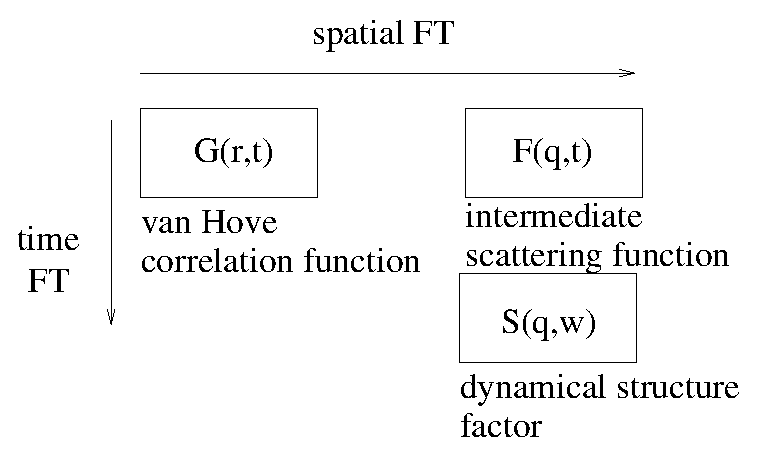
\includegraphics[width=0.9\textwidth]{figures/GFS.eps}
  \end{center}
\caption{Relations between dynamical functions using space, time, wavevector and energy variables.}
\label{f:GFS}
\end{figure}

In the case of a homogeneous and classical liquid, the \emph{van Hove correlation function}, which describes the time and space correlations in the liquid, can be written \cite{Egelstaff67,squires}:
\begin{equation} \label{eq:vanhove}
G(\vec{r},t) = \frac{1}{N} \sum_{i=1}^N \sum_{j=1}^N  \langle\delta[\vec{r} + \vec{r}_i(0) - \vec{r}_j(t)]\rangle
\end{equation}
with $\vec(r)$ and $t$ being the position and time of the atom distribution in the liquid.
Using the particule-density function $\rho(\vec(r),t)$, the function $G$ can be rewritten:
\begin{equation} \label{eq:vanhove-rho}
G(\vec{r},t) = \frac{\langle \rho(0,0) \rho(\vec{r},t)\rangle}{\rho}
\end{equation}

On the experimental point of view, one usually refers to the \emph{dynamical structure factor} $S(q,\omega)$, which is the double Fourier-transform in space and time of the van Hove correlation function $G(r,t)$:
\begin{eqnarray} \label{eq:sqw-rho}
S(q,\omega) &= \frac{1}{2\pi}\int_{-\infty}^{\infty} F(\vec{q},t) e^{-i\omega t} dt \nonumber \\
            &= \frac{1}{2\pi N} \int_{-\infty}^{\infty} \langle \hat\rho^*(\vec{q},0) \hat\rho(\vec{q},t) \rangle e^{-i\omega t} dt.
\end{eqnarray}
where $\hat\rho(\vec{q}, t)$ is the spatial Fourier transform of the density $\rho(\vec{r},t)$, and the \emph{intermediate scattering function} $F$ is the time correlation function of $\hat\rho$:
\begin{eqnarray}
F(\vec{q},t) &= \frac{1}{N} \langle \hat\rho^*(\vec{q},0)  \hat\rho(\vec{q},t) \rangle \nonumber \\
                    &= \frac{1}{N} \sum_{i=1}^N \sum_{j=1}^N \langle e^{i \vec{q}.(\vec{r}_j(t) - \vec{r}_i(0))} \rangle
\end{eqnarray}
Some easely measureable quantities in a liquid are the \emph{pair correlation function} $g(r)$ and the \emph{structure factor} $S(q)$, defined as:
\begin{eqnarray}
\rho g(\vec{r}) &= \frac{1}{N} \sum_{i=1}^N \sum_{j \neq i} \langle \delta(\vec{r}+\vec{r}_i-\vec{r}_j) \rangle \\
S(\vec{q}) &=1 + \rho \int_V [g(\vec{r})-1] e^{i\vec{q}.\vec{r}} d\vec{r} \\
           &=1 + \rho \int_{0}^{\infty} [g(r)-1] \frac{\sin(qr)}{qr} 4 \pi r^2 dr {\rm in isotropic materials}
\end{eqnarray}
Both $g(r)$ and $S(q)$ converge to unity for large $r$ and $q$ values respectively, and they are representative of the atoms spatial distribution.


Following Squires (\cite{squires}, p63), the neutron differential scattering cross section for both coherent and incoherent processes is
\begin{equation}
\frac{d^2\sigma}{d\Omega dE_f} = \frac{\sigma}{4\pi}\frac{k_f}{k_i} N S(q, \omega)
\end{equation}
with usual notations. The unit of the dynamical structure factor $S$ is an inverse energy.

\subsection{How does a neutron interact with the material ?}


\subsection{The implementation}
\subsubsection{Choosing the interaction position}
\subsubsection{Choosing the type of interaction}
\subsubsection{Choosing the $q$ and $\omega$ transfert}